\documentclass[10pt,a4paper]{article}
\usepackage{fontspec}
\usepackage{amsmath}
\usepackage{amsfonts}
\usepackage{amssymb}
\usepackage{graphicx}
\usepackage[left=1.00in, right=1.00in, top=1.00in, bottom=1.00in]{geometry}
\usepackage[colorlinks=true,
			linkcolor=blue]{hyperref}
\usepackage{cleveref}
\usepackage{minted}
\usepackage{lmodern}

\begin{document}
	\title{Assignment 2:\\Comparison of Sheath Conditions}
	\author{Daniel Celis Garza}
	\date{\today}
	\maketitle
	
	The normalised ion velocity at the start of the sheath, $v_{s}$, was varied between 1 and 2 with 0.5 step increments. We defined an array $\mathbf{x_{wall}} = \mathbf{x} - x(J=0)$, where $\mathbf{x}$ is the unadjusted $x$-array and $x(J=0)$ the value of $x$ where $J=0$ as found via interpolation. \Cref{fig:1} shows the plot of $J$ as a function of $x_{wall}$.
	\begin{figure}[H]
		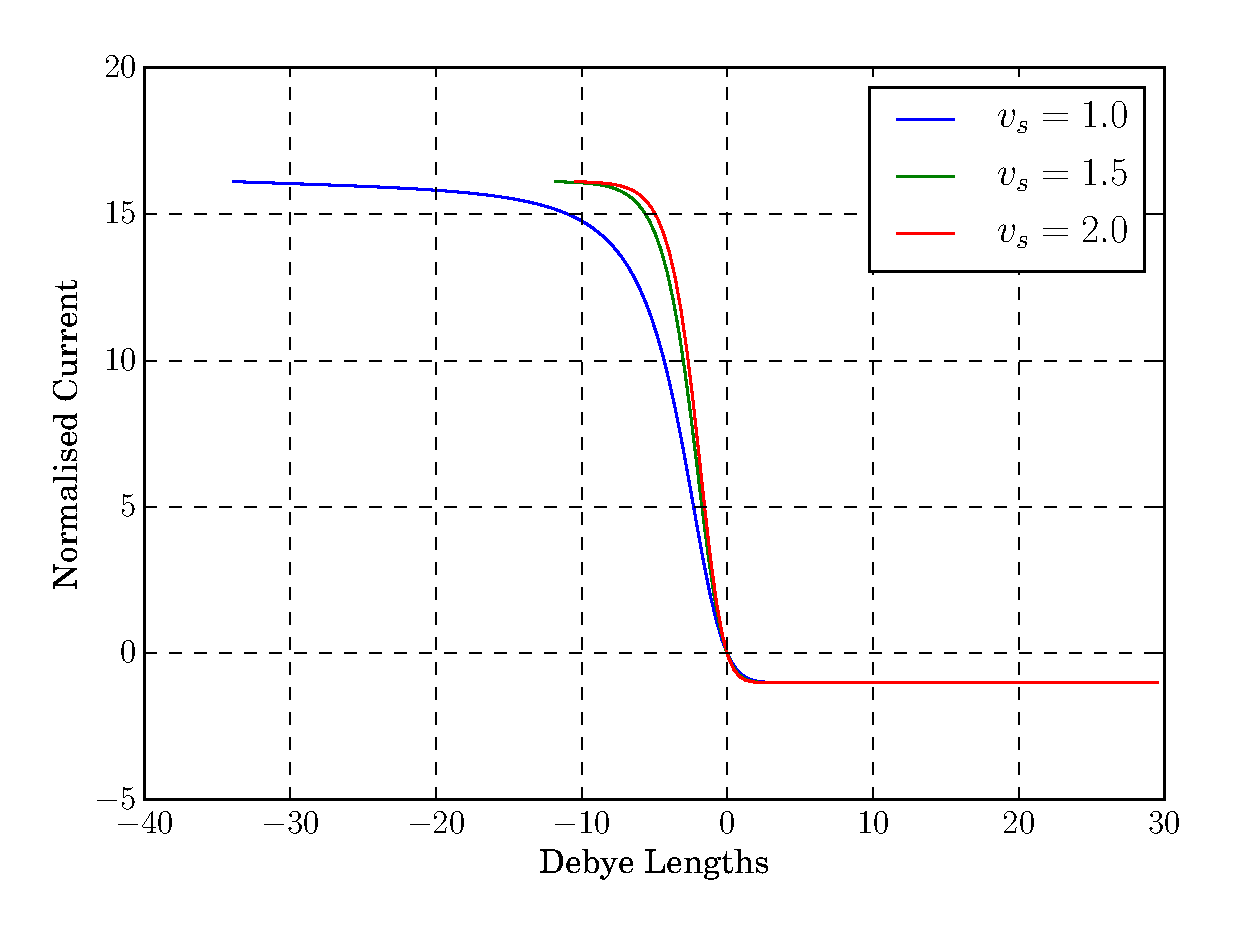
\includegraphics[width=\textwidth]{changevs.eps}
		\caption{$J$ as a function of $x_{wall}$.}\label{fig:1}
	\end{figure}
	
	The code was implemented using an object-oriented approach for easy expandability.
	\inputminted[linenos = true,
				 breaklines, 
				 breakanywhere]{python}{dcg513_2.py}
\end{document}